\section{Motivation}
\begin{frame}{Structural Attacks}{Invariant Subspaces}
    \begin{block}{Invariant Subspaces~\cite{C:GAAZ11} (Crypto 2011)}
        Let $U$ be a subspace of $\F_2^n$, and $F : \F_2^n \to \F_2^n$.
        We write $\coset{U}{a} \through{F} \coset{U}{b}$, if
        \begin{equation*}
            \exists a : \exists b : F(\coset{U}{a}) = \coset{U}{b}
        \end{equation*}
    \end{block}
    \begin{block}{Main Idea}
    \begin{center}
        \begin{tikzpicture}[scale=0.8]
            \tikzstyle{every node}=[transform shape];

            \node (left1-space) [draw,rectangle,thick,rounded corners,minimum width=3cm,minimum height=4cm,fill=white] at (-8,0)
            {\begin{tikzpicture}[scale=0.7]
                    \node (u) [draw,rectangle,thick, fill=gray!20]
                    {\begin{tikzpicture}[scale=1.2]
                            \draw[rounded corners=2pt]
                                (-1.2,1.9) -- (-1,1.9) -- (-0.9,1.7) -- (-1.1,1.2) -- (-1,0.9) -- (-1.4,0.6) -- (-1.1,0.1) -- (-1.2,-0.4) -- (-1.5,-0.2) -- (-1.8,-0.3) -- (-2.2,-0.6) -- (-2.7,-0.3) -- (-2.2,0.8) -- (-2.4,1) -- (-2.6,1) -- (-2.7,1.2) -- (-2.6,1.8) -- (-2.3,1.8) -- (-2.1,2.2) -- (-1.6,2.3) -- (-1.4,2.3) -- (-1.4,2.1) -- (-1.3,2) -- (-1.2,1.9);
                    \end{tikzpicture}};
            \end{tikzpicture}};

            \node (right1-space) [draw,rectangle,thick,rounded corners,minimum width=3cm,minimum height=4cm,fill=white] at (-4,0)
            {\begin{tikzpicture}[scale=0.7]
                    \node (u) [draw,rectangle,thick] {%
                        \begin{tikzpicture}[scale=1.2]
                            \draw[rounded corners=2pt, fill=gray!20]
                                (-1.2,1.9) -- (-1,1.9) -- (-0.9,1.7) -- (-1.1,1.2) -- (-1,0.9) -- (-1.4,0.6) -- (-1.1,0.1) -- (-1.2,-0.4) -- (-1.5,-0.2) -- (-1.8,-0.3) -- (-2.2,-0.6) -- (-2.7,-0.3) -- (-2.2,0.8) -- (-2.4,1) -- (-2.6,1) -- (-2.7,1.2) -- (-2.6,1.8) -- (-2.3,1.8) -- (-2.1,2.2) -- (-1.6,2.3) -- (-1.4,2.3) -- (-1.4,2.1) -- (-1.3,2) -- (-1.2,1.9);
                        \end{tikzpicture}
                    };
            \end{tikzpicture}};

            \draw[-latex] (-8,0.5) to [bend left] node[above]{$F$} (-4,0.5);
            \draw[-latex] (-4.75,-0.5) to [bend left] node[below]{$F^{-1}$} (-7.25,-0.5);
        \end{tikzpicture}
    \end{center}
    \end{block}
\end{frame}

\begin{frame}{Structural Attacks}{Subspace Trail Cryptanalysis}
    \begin{block}{Subspace Trail Cryptanalysis~\cite{ToSC:GraRecRon16} (Last Year's FSE)}
        Let $U$, $V$ be subspaces of $\F_2^n$, and $F : \F_2^n \to \F_2^n$.
        We write $U \through{F} V$, if
        \begin{equation*}
            \forall a : \exists b : F(\coset{U}{a}) \subseteq \coset{V}{b}
        \end{equation*}
    \end{block}
    We restrict ourselves to \emph{essential} subspace trails.
    \begin{block}{Main Idea}
        \centering
        \vspace{0.25em}
        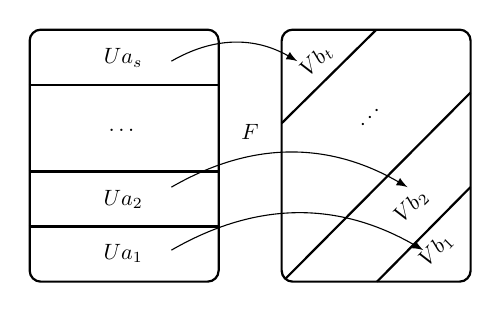
\begin{tikzpicture}[scale=0.8]
            \tikzstyle{every node}=[transform shape];

            \node (left2-space) [draw,rectangle,thick,rounded corners,minimum width=3cm,minimum height=4cm,fill=white] at (1,0) {};
            \draw[thick] (left2-space.west)+(0,1.125cm) -- node[above, yshift=1.5mm] {$\coset{U}{a_s}$} +(3cm,1.125cm);
            \draw[thick] (left2-space.west)+(0,-0.25cm) -- node[above, yshift=5mm] {\dots} +(3cm,-0.25cm);
            \draw[thick] (left2-space.west)+(0,-1.125cm) -- node[above, yshift=1.5mm] {$\coset{U}{a_2}$}
                                                            node[below, yshift=-1.5mm] {$\coset{U}{a_1}$} +(3cm,-1.125cm);

            \node (right2-space) [draw,rectangle,thick,rounded corners,minimum width=3cm,minimum height=4cm,fill=white] at (5,0) {};
            \draw[thick] (right2-space.north)+(0pt,-0.5pt) -- node[above, yshift=0.5mm, rotate=45] {$\coset{V}{b_t}$} +(-1.5cm,-1.5cm);
            \draw[thick] (right2-space.east)+(-0.5pt,1cm) -- node[above, yshift=10mm, rotate=45] {\dots} +(-3cm+1.25pt,-2cm+1.25pt);
            \draw[thick] (right2-space.east)+(-0.5pt,-5mm) -- node[above, yshift=2.5mm, rotate=45] {$\coset{V}{b_2}$}
                                                        node[below, yshift=-0.5mm, rotate=45] {$\coset{V}{b_1}$} +(-1.5cm,-2cm);

            \node (right-f) at (3,0.375) {$F$};

            \draw[-latex] (1.75,-0.5) to [bend left] (5.5,-0.5);
            \draw[-latex] (1.75,-1.5) to [bend left] (5.75,-1.5);
            \draw[-latex] (1.75,+1.5) to [bend left] (3.75,+1.5);
        \end{tikzpicture}
    \end{block}
\end{frame}

\begin{frame}{The Problem}{How to search efficiently for Subspace Trails?}
    \visible<1->{%
    \begin{alertblock}{Security against Subspace Trails?}
        Given the round function $F : \F_2^n \to \F_2^n$ of an SPN cipher, prove the resistance against subspace trail attacks!
    \end{alertblock}
    }
    \visible<2->{%
    \begin{block}{Main problem: Too many possible starting points.}
        Already for initially one-dimensional subspaces there are $2^n$ possibilities.
    \end{block}
    }
    \visible<2->{%
    \begin{block}{Can't we just activate a single S-box and check to what this leads us?}
        \visible<3->{%
        \begin{center}
            The short answer is:\\No!\footnote{\visible<3->{The long answer is this talk.}}
        \end{center}
        }
    \end{block}
    }
\end{frame}

\section{Intuition}
\begin{frame}{Outline}{}
    \begin{block}{Outline}
        \vspace{0.5em}
        \tableofcontents
    \end{block}
\end{frame}

\begin{frame}{Preliminaries, Notations}
    \begin{block}{Subspace Complement}
        If $U$ is a subspace of $\F_2^n$, we denote by $U^\perp$ it's \emph{complement}:
        \vspace{-0.5em}
        \begin{equation*}
            U^\perp \coloneqq \set{u \in \F_2^n \given \forall x \in U: \angles{x, u} = 0}
            \vspace*{-0.5em}
        \end{equation*}
    \end{block}
    \begin{block}{Derivative}
        Let $F : \F_2^n \to \F_2^n$.
        We denote the \emph{derivative of $F$ in direction $u$} by
        \vspace*{-0.5em}
        \begin{equation*}
            \Delta_u(F)(x) \coloneqq F(x) + F(x + u)
            \vspace*{-0.5em}
        \end{equation*}
    \end{block}
    \begin{block}{Linear Structure}
        Let $F : \F_2^n \to \F_2^n$.
        Then $(\alpha, u)$ is called a \emph{linear structure}, if
        \vspace*{-0.5em}
        \begin{equation*}
            \exists c \in \F_2 : \forall x \in \F_2^n : \angles{\alpha, \Delta_u(F)(x)} = c
            \vspace*{-0.5em}
        \end{equation*}
    \end{block}
\end{frame}

\begin{frame}{Intuition}{The Image of the Derivative is in the Subspace}
    \begin{minipage}{0.99\textwidth}
    \begin{lemma}
        \vspace{0.5em}
        Let $U \through{F} V$ be a subspace trail.
        Then
        \begin{equation*}
            \forall u \in U : \mathrm{Im}\parens{\Delta_u(F)} \subseteq V.
        \end{equation*}
    \end{lemma}
    \end{minipage}
    \begin{columns}
        \hspace{4pt}
        \begin{column}{0.475\textwidth}
            \begin{block}{Remember:}
                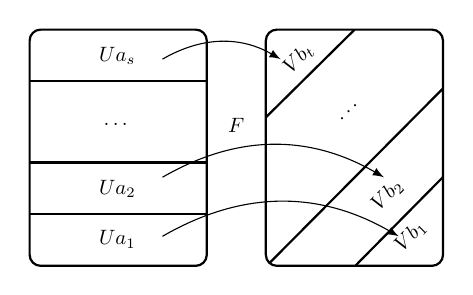
\begin{tikzpicture}[scale=0.75]
                    \tikzstyle{every node}=[transform shape];

            \node (left2-space) [draw,rectangle,thick,rounded corners,minimum width=3cm,minimum height=4cm,fill=white] at (1,0) {};
            \draw[thick] (left2-space.west)+(0,1.125cm) -- node[above, yshift=1.5mm] {$\coset{U}{a_s}$} +(3cm,1.125cm);
            \draw[thick] (left2-space.west)+(0,-0.25cm) -- node[above, yshift=5mm] {\dots} +(3cm,-0.25cm);
            \draw[thick] (left2-space.west)+(0,-1.125cm) -- node[above, yshift=1.5mm] {$\coset{U}{a_2}$}
                                                            node[below, yshift=-1.5mm] {$\coset{U}{a_1}$} +(3cm,-1.125cm);

            \node (right2-space) [draw,rectangle,thick,rounded corners,minimum width=3cm,minimum height=4cm,fill=white] at (5,0) {};
            \draw[thick] (right2-space.north)+(0pt,-0.5pt) -- node[above, yshift=0.5mm, rotate=45] {$\coset{V}{b_t}$} +(-1.5cm,-1.5cm);
            \draw[thick] (right2-space.east)+(-0.5pt,1cm) -- node[above, yshift=10mm, rotate=45] {\dots} +(-3cm+1.25pt,-2cm+1.25pt);
            \draw[thick] (right2-space.east)+(-0.5pt,-5mm) -- node[above, yshift=2.5mm, rotate=45] {$\coset{V}{b_2}$}
                                                        node[below, yshift=-0.5mm, rotate=45] {$\coset{V}{b_1}$} +(-1.5cm,-2cm);

                    \node (right-f) at (3,0.375) {$F$};

                    \draw[-latex] (1.75,-0.5) to [bend left] (5.5,-0.5);
                    \draw[-latex] (1.75,-1.5) to [bend left] (5.75,-1.5);
                    \draw[-latex] (1.75,+1.5) to [bend left] (3.75,+1.5);
                \end{tikzpicture}
            \end{block}
        \end{column}
        \begin{column}{0.475\textwidth}
            \begin{block}{Proof}
                \vspace{0.5em}
                Let $U \through{F} V$, then for every $u \in U$
                \begin{align*}
                    x \in \coset{U}{x} &\through{F} F(x) \in \coset{V}{b}, \\
                    x+u \in \coset{U}{x} &\through{F} F(x+u) \in \coset{V}{b},
                \end{align*}
                implying $F(x) + F(x + u) \in V$.
                \qed{}
                \vspace{0.5em}
            \end{block}
        \end{column}
    \end{columns}
\end{frame}

\section{Algorithm}
\begin{frame}{Approach to the Algorithm}
    \begin{columns}
        \begin{column}{0.6\textwidth}
            \begin{block}{SPN Structure\vphantom{y}}
                \vspace{0.5em}
                \begin{tikzpicture}
                \foreach \z in {0,1,2,3} {%
                    \node[] (i\z) at ($(-0.25, \z*3em)+(0,0.35)$) {};
                    \node[] (o\z) at ($\z*(0, 3em)+(18.25em,0.35)$) {};
                    \draw[thick,solid] (i\z) -- (o\z.center);
                }

                %% SBoxes
                \foreach \z in {0,1,2,3} {%
                    \node[draw,thick,solid,minimum width=2em,minimum height=2.75em,fill=white] (sl\z) at ($(0,\z*3em) + (2em,1.1em)$) {$S$};
                }
                %% Permutation Box
                \node[draw,thick,solid,minimum width=2em,minimum height=11.75em,fill=white] (p1) at ($(1.125em,0) + (3.125em,5.6em)$) {$P$};

                %% Round Dashed Box
                \draw[thick,dashed] ($(sl3.north west)+(-0.25em,0.15)$) rectangle ($(p1.south east)+(0.35em,-0.15)$);


                %% SBoxes
                \foreach \z in {0,1,2,3} {%
                    \node[draw,thick,solid,minimum width=2em,minimum height=2.75em,fill=white] (sm\z) at ($(2.125,\z*3em) + (2em,1.1em)$) {$S$};
                }
                %% Permutation Box
                \node[draw,thick,solid,minimum width=2em,minimum height=11.75em,fill=white] (p2) at ($(5.5125em,0) + (4.8em,5.6em)$) {$P$};

                %% Round Dashed Box
                \draw[thick,dashed] ($(sm3.north west)+(-0.25em,0.15)$) rectangle ($(p2.south east)+(0.35em,-0.15)$);


                %% SBoxes
                \foreach \z in {0,1,2,3} {%
                    \node[draw,thick,solid,minimum width=2em,minimum height=2.75em,fill=white] (sr\z) at ($(4.25,\z*3em) + (2em,1.1em)$) {$S$};
                }
                %% Permutation Box
                \node[draw,thick,solid,minimum width=2em,minimum height=11.75em,fill=white] (p3) at ($(11.525em,0) + (4.8em,5.6em)$) {$P$};

                %% Round Dashed Box
                \draw[thick,dashed] ($(sr3.north west)+(-0.25em,0.15)$) rectangle ($(p3.south east)+(0.35em,-0.15)$);
                \end{tikzpicture}
                \vspace{0.5em}
            \end{block}
        \end{column}
        \begin{column}{0.35\textwidth}
            \begin{block}{Easy parts}
                \vspace{4mm}
                \begin{itemize}
                    \item Given a starting subspace, computing the trail is easy.
                    \item The effect of the linear layer $P$ to a subspace $U$ is clear:
                          \begin{equation*}
                              U \through{P} P(U)
                          \end{equation*}
                \end{itemize}
                \vspace{4mm}
            \end{block}
        \end{column}
    \end{columns}
    \begin{block}{How to reduce the number of starting points?}
        Two possibilities, depending on the S-box $S$.
    \end{block}
\end{frame}

\begin{frame}{Possibility I}{The short one}
    \begin{block}{Observation}
        \vspace{0.25em}
        For an S-box $S$ and $U \through{S} V$, because of the above lemma,
        \begin{align*}
            \forall x, \forall u \in U&: \Delta_u(F)(x) \in V \\
            \Rightarrow \forall \alpha \in V^\perp : \forall x, \forall u \in U &: \angles{\alpha, \Delta_u(F)(x)} = 0.
        \end{align*}
        Thus, $V^\perp$ consists of the linear structures of $S$.
    \end{block}
    \begin{theorem}
        Let $F : \F_2^{kn} \to \F_2^{kn}$ be an S-box layer that applies $k$ S-boxes with no non-trivial linear structures in parallel.
        Then every essential subspace trail $U \through{F} V$ is of the form
        \begin{equation*}
            U = V = U_1 \times \cdots \times U_k,
        \end{equation*}
        where $U_i \in \set{\set{0}, \F_2^n}$.
    \end{theorem}
\end{frame}

\begin{frame}{Possibility I}{Algorithm}
    \begin{block}{Algorithm}
        Simply activate single S-boxes.
    \end{block}
    \begin{block}{The problem with S-boxes that have linear structures}
    \end{block}
\end{frame}

\begin{frame}{Possibility II}{The long one}
    \begin{block}{Observation}
        \vspace{0.25em}
        If $U_1 \through{F} U_2$ is a subspace, so is $V_1 \through{F} V_2$:
        \begin{equation*}
        \begin{aligned}
            & U_1 & \stackrel{F}{\longrightarrow}\ &\ U_2 \\
            & \rotatebox[origin=c]{90}{$\subseteq$} & &\ \rotatebox[origin=c]{90}{$\subseteq$} \\
            & V_1 & \stackrel{F}{\longrightarrow}\ &\ V_2
        \end{aligned}
        \end{equation*}
    \end{block}
\end{frame}
